%% Based on a TeXnicCenter-Template by Gyorgy SZEIDL.
%%%%%%%%%%%%%%%%%%%%%%%%%%%%%%%%%%%%%%%%%%%%%%%%%%%%%%%%%%%%%

%------------------------------------------------------------
%
\documentclass[a4paper,12pt,leqno, notitlepage]{article}%
%Options -- Point size:  10pt (default), 11pt, 12pt
%        -- Paper size:  letterpaper (default), a4paper, a5paper, b5paper
%                        legalpaper, executivepaper
%        -- Orientation  (portrait is the default)
%                        landscape
%        -- Print size:  oneside (default), twoside
%        -- Quality      final(default), draft
%        -- Title page   notitlepage, titlepage(default)
%        -- Columns      onecolumn(default), twocolumn
%        -- Equation numbering (equation numbers on the right is the default)
%                        leqno
%        -- Displayed equations (centered is the default)
%                        fleqn (equations start at the same distance from the right side)
%        -- Open bibliography style (closed is the default)
%                        openbib
% For instance the command
%           \documentclass[a4paper,12pt,leqno]{article}
% ensures that the paper size is a4, the fonts are typeset at the size 12p
% and the equation numbers are on the left side
%
\usepackage{amsmath}%
\usepackage{amsfonts}%
\usepackage{amssymb}%
\usepackage{graphicx}
\usepackage[utf8]{inputenc}
\usepackage[magyar]{babel}
%-------------------------------------------
\frenchspacing
\sloppy

\begin{document}

\title{Agilis módszertan bevezetése}
\author{Horváth András \\ Széchenyi István Egyetem, Győr}
\date{2019. november 13}
\maketitle

\begin{abstract}

Ez a dolgozat az IT projekmenedzsment tárgy teljesítéséhez készült. A dolgozatban összehasonlítom a kalsszikus és az agilis szoftver\-fejlesztési folya\-matot. Bemutatom ezek szereplőit, metódusait, alkalmazási területeit.

Ezután áttekintem a projektmenedzsment szereplőit és folyamatát. Célom bemutatni, hogy egy szoftverfejlsztéssel foglalkozó hogyan kerülhet bevezetésre az agilis módszertan. Legvégül kitérek arra kérdésre, hogy lehet-e átfedés vagy valamilyen kapcsolat a projekt-menedzseri feladatok és az agilis szoftver\-fejlesztés szerepkörei között.
\end{abstract}

\section{Szoftver\-fejlesztési módszerek}
\label{sec:s}

A dolgozat elején kettő, alapvetően különböző szoftver\-fejlesztési módszert tekintünk át. A két módszer között lényeges szemléletbeli különbségek vannak.

\subsection{Klasszikus szoftver\-fejlesztés}
\label{sec:Klasszikus}

Klasszikus szoftver\-fejlesztés alatt legtöbben a vízesés modellt értik. Ez a módszer régen nagyon elterjedt volt manapság viszont szinte elképzelhetetlen a használata. Ennek oka a módszer egyenes munkafolyamata és szigorúsága.

%D:/SZE/it_projmen/latex/
\begin{figure}[htb]
	\centering
		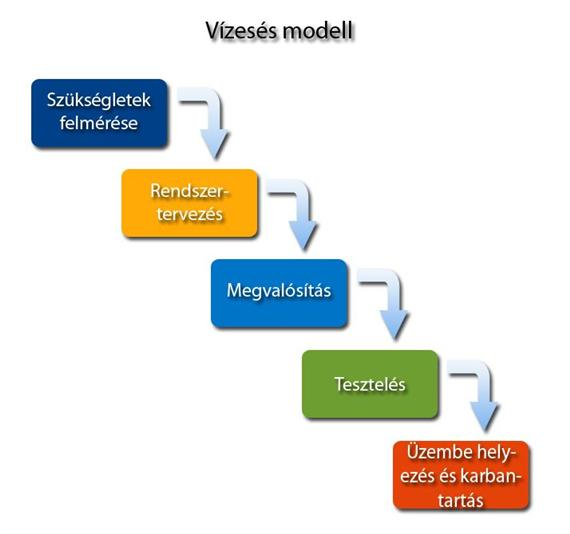
\includegraphics[width=0.95\textwidth]{images/waterfall.jpg}
	\caption{A vízesés modell fázisai \cite{waterfall_image}}
	\label{fig:waterfall}
\end{figure}


\cite{waterfall}


\subsection{Agilis szoftver\-fejlesztés}



\section{A szoftver\-fejlesztés mint projekt}


\bibliography{biblio}{}
\bibliographystyle{plain}

\end{document}
